\documentclass{beamer}
\renewcommand\thesection{\arabic{section}}
\newcommand{\myfont}{\rmfamily\normalsize\upshape\mdseries}
\newcommand{\degree}{^\circ}
\title{\sffamily Review II(Slides 62 - 108)}
\subtitle{\textbf{Numbers}\\ We define everything as they now defined for some good reasons...}
\institute[UM-SJTU JI]{University of Michigan-Shanghai Jiao Tong University Joint Institute}
\author{HamHam}
\usepackage{graphicx}
\usepackage{picinpar}
\usepackage{indentfirst}
\usepackage{chemformula}
\usepackage{geometry}
\usepackage{subfigure}
\usepackage{appendix}
\usepackage{amsfonts,amsmath,amssymb}
\usepackage{enumerate}
\usepackage{float}
\usepackage{geometry}
\usepackage{latexsym}
\usepackage{listings}
\usepackage{multicol,multirow,multido}
\usepackage{tabularx}
\usepackage{ulem}
\usepackage{tikz}
\usepackage{xcolor}
\usepackage{cite}
\usepackage{setspace}
\usepackage{hyperref}
\usepackage{textpos}
\usepackage{booktabs}

\usetheme[dove]{Boadilla}
\usecolortheme{dolphin}
\useoutertheme{miniframes}
\begin{document}
    \usebackgroundtemplate{\tikz\node[opacity=0.3]{
    
\includegraphics[width=\paperwidth,
    height=\paperheight]{hamster.jpg}
    };}
\begin{titlepage}
    \begin{center}
        VV186 - Honors Mathmatics II
    \end{center}
\end{titlepage}
\myfont
\section{Natural Numbers}
\begin{frame}
    \frametitle{Natural Numbers}
    \hspace{1em}
The natural numbers can be constructed using the 
\textbf{Peano Axioms} and set theory, 
which will be one of the main topics in \textbf{Ve203 Discrete Mathematics}. 
The Peano Axioms is also the theoretical basis of \textbf{mathematical induction}.
But here in vv186 we don't care much and just simply denote the set of natural numbers by $\mathbb{N}$ and define it as:
\begin{equation*}
    \mathbb{N}=\{0,1,2,3,4,\dots\}
\end{equation*}
    We will have following \textbf{properties} we simply take it as \emph{axioms}.
    \begin{table}
        \centering
        \resizebox{11cm}{!}{%
        \begin{tabular}{ccc}
            \toprule
            $Porperties$& \multicolumn{1}{c}{Addition} &\multicolumn{1}{c}{Multiplication} \\
            \midrule
            $Associativity$ & $a+(b+c)=(a+b)+c$ & $a\cdot (b\cdot c)=(a\cdot b)\cdot c$ \\
            $Existence$ & $a+0=0+a=a$ & $a\cdot 1=1\cdot a=a$ \\
            $Commutativity$ & $a+b=b+a$  & $a\cdot b=b\cdot a $\\
            $Distributivity$ & \multicolumn{2}{c}{$a\cdot (b+c)=a\cdot b+a\cdot c$} \\
            \bottomrule
        \end{tabular}%
        }
    \end{table}
\end{frame}

\begin{frame}
    \frametitle{Mathematical Induction}
\hspace{1em} Let $A$ be a statement that has to do with \textbf{natural numbers}. We denote 
the statement with respect to a specific number $n$ as $A(n)$. \\
\vspace{1em}
There are two types of Mathematical Induction.\\
\vspace{1em}
\textbf{Mathematical Induction I}
\begin{enumerate}
    \item $A(n_0)$ is true
    \item $A(n+1)$ is true whenever $A(n)$ is true for $n \geq n_0$
\end{enumerate}
\vspace{1em}
\textbf{Mathematical Induction II}
\begin{enumerate}
    \item $A(n_0)$ is true
    \item $A(k+1)$ is true whenever $A(n)$ is true for all $n_0\leq n\leq k$
\end{enumerate}
\end{frame}

\myfont
\begin{frame}
    \frametitle{Proof of Mathematical Induction II}
    \hspace*{1em}
    Suppose that a statement $A$ holds for mathematical induction II, but there is 
    a set $F \subseteq\mathbb{N}$ such that $\forall m \in F$, $A(m)$ doesn't hold.
    i.e., $A$ does not hold for all $n \in \mathbb{N}$. \\
    $\Rightarrow$ There is a smallest number $m_0 \in F$ such that $A(m_0)$ doesn't hold
    (because the set $\mathbb{N}$ is well-ordered).\\
    \hspace{1em} However, $A(m_0-1)$ holds, according to our induction, $A(m_0)$ holds.
    This leads to a contradiction.\\
    \hspace{1em} Thus mathematicl induction II holds.
\end{frame}
\begin{frame}
    \frametitle{Application of Mathematical Induction¿}
    \hspace{1em}
    A strange example shared by Horst. What's going wrong?
    \begin{figure}
        \centering
        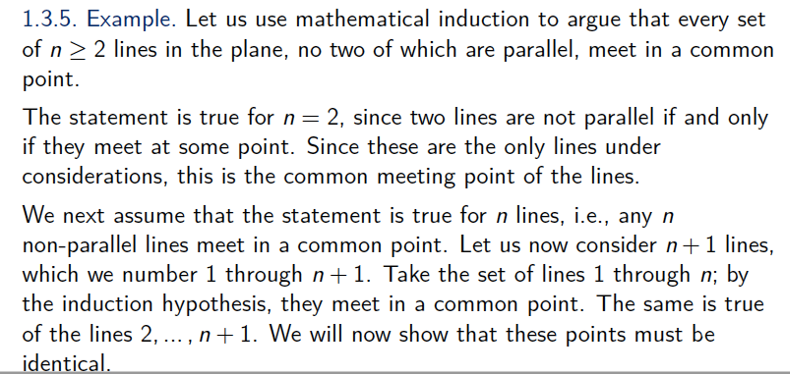
\includegraphics[width=1\textwidth]{induction1.png}
    \end{figure}
   
\end{frame}
\begin{frame}
    \frametitle{Application of Mathematical Induction¿}
    \hspace{1em}
    A strange example shared by Horst. What's going wrong?
    \begin{figure}
        \centering
        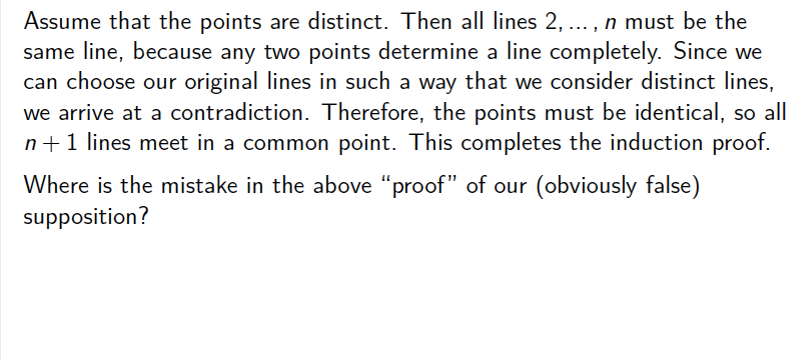
\includegraphics[width=1\textwidth]{induction2.png}
    \end{figure}
   
\end{frame}
\begin{frame}
    \frametitle{How to use Induction}
    \begin{itemize}
        \item Examine the complexity of the problem, because using induction is sometimes much more
            complicated than using a direct method to prove a statement.
        \item Determine the initial condition (i.e. $n_0$) for your induction proof.
        \item Decide the part of the proof that you use induction and which induction you want to use.
        \item Make a short test of your method on draft paper to see whether it works and is easy to write down.
    \end{itemize}
    \begin{itemize}
        \item[!] \textcolor{red}{One of the solid example is Slides 67-70, the proof of Binomial Formula, please check it!}
    \end{itemize}
\end{frame}
\section{Rational Nums etc.}
\begin{frame}
    \frametitle{Rational Numbers}
    \hspace{1em}
    We define that the set of rational numbers is 
    \begin{equation*}
        \mathbb{Q}=\{\frac{p}{q}:p,q\in \mathbb{Z}\wedge q \neq 0\}
    \end{equation*}
    together with the following properties(P1-P9). You will learn this in 
    \textbf{Ve203 Discrete Mathematics}.
    \begin{table}
        \centering
        \resizebox{10cm}{!}{%
        \begin{tabular}{cccc}
            \toprule
            $Porperties$& \multicolumn{1}{c}{Addition} & &\multicolumn{1}{c}{Multiplication} \\
            \midrule
            $Associativity$ & $a+(b+c)=(a+b)+c$ && $a\cdot (b\cdot c)=(a\cdot b)\cdot c$ \\
            \\
            $Neutral Element$ & $a+0=0+a=a$ && $a\cdot 1=1\cdot a=a$ \\
            \\
            $Commutativity$ & $a+b=b+a$  && $a\cdot b=b\cdot a $\\
            \\
            $Inverse Element$& $(-a)+a=a+(-a)=0$ && $a\cdot a^{-1}=a^{-1}\cdot a=1$ \\
            \\
            $Distributivity$ & \multicolumn{3}{c}{$a\cdot (b+c)=a\cdot b+a\cdot c$} \\
            \bottomrule
        \end{tabular}%
        }
    \end{table}
\end{frame}    

\begin{frame}
    \frametitle{Trichotomy law}
    \hspace{1em}
    There are still three axioms we will define, and together with the nine axioms above, 
we build our rational numbers $\mathbb{Q}$.\\
    \vspace{1em} 
    \hspace{1em}   
    We assume that we know what a strictly positive rational number is, then we know we can find such 
    a set $P$ with the property that :
    \hspace{1em}
    \begin{enumerate}
        \item $a=0$
        \item $a\in P$
        \item $-a\in P$
    \end{enumerate}
which is so-called \textbf{trichotomy law}.\\
\hspace{1em}
Further more, we assume that the set of positive number $P$ is 
\itshape closed under addition and multiplication.\\
\myfont
\end{frame}
\begin{frame}
    \frametitle{The Square Root Problem}
    \hspace{1em}
    Let $M=\{t \in \mathbb{R} : t>0 \wedge t^2>x \}, y=\inf M.$
    We want to prove that $y^2=x$ by showing that $y^2 > x$ and $y^2<x$ 
    lead to contradictions.
    \begin{figure}
        \centering
        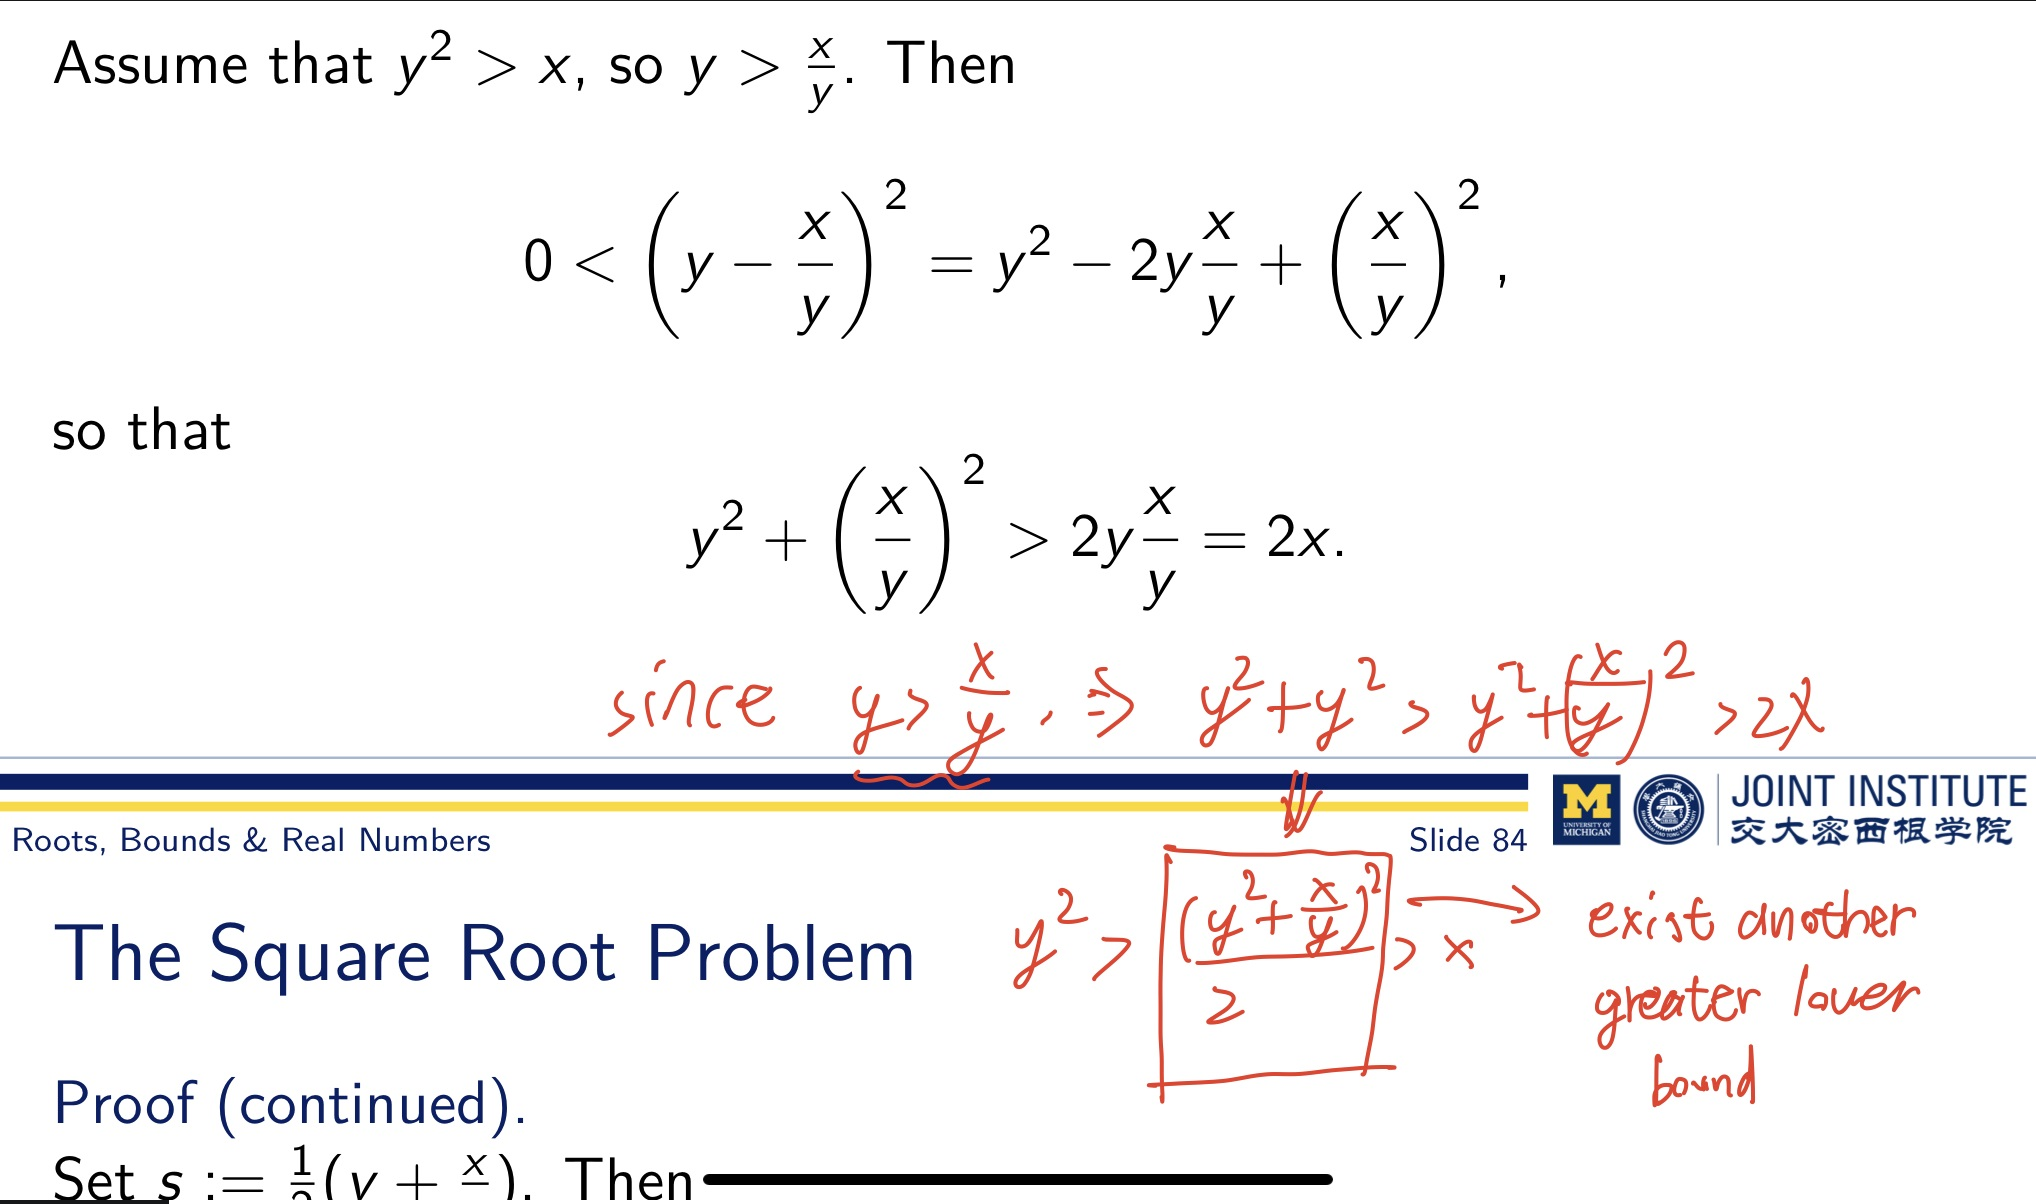
\includegraphics[width=0.8\textwidth]{square.jpg}
    \end{figure}
\end{frame}
\begin{frame}
    \frametitle{Complex Numbers}
    \hspace{1em}
    In Vv186, you just need to know how to perform basic complex numbers' computation 
    and some basic properties.
    Here, we just list some basic computation rules and formulas.\\
    Given $z_1=(a_1,b_1)$ and $z_2=(a_2,b_2)$,
\begin{itemize}
    \item $z_1+z_2=(a_1,b_1)+(a_2,b_2)=(a_1+a_2,b_1,b_2)$
    \item $z_1\cdot z_2=(a_1,b_1)\cdot (a_2,b_2)=(a_1a_2-b_1b_2,a_1b_2-a_2b_1)$
    \item $c\cdot z_1=c(a_1,b_2)=(ca_1,cb_1), c\in \mathbb{R} $
    \item $\bar{z_1}=(a_1,-b_1)$
    \item $|z_1|^2=a_1^2+b_1^2=z_1\bar{z_1}$
    \item Re $z_1= \frac{z_1+\bar{z_1}}{2}$
    \item $($Im $z_1 )i= \frac{z_1-\bar{z_1}}{2}$
\end{itemize}
\end{frame}
\section{Sets \& Points}
\begin{frame}
    \frametitle{Interval}
    Recall...\\
    \begin{itemize}
        \item Open interval 
        \item Closed interval 
        \item Half-open (or half-closed) interval
    \end{itemize}
    \vspace{2em}
    \hspace{1em}
    $"("$ and $ ")"=$ open \\
    \hspace{1em}
    $"["$ and $ "]"=$ closed \\
\end{frame}
\begin{frame}
    \frametitle{Sets \& Points}
    Recall the following definition and try to write down their \textbf{notation}...\\
    \begin{itemize}
        \item Interior point
        \item Exterior point
        \item Boundary point
        \item Accumalation point
        \item Open Set
        \item Closed set
        \item Closure 
    \end{itemize}
    \vspace{0.5em}
    Tips:\\
    \begin{itemize}
        \item \textbf{Remember the definitions!}\\
        \item \textbf{Draw the pictures!}\\
        \item \textbf{Pay attention to some speacial cases!}
    \end{itemize}
\end{frame}
\begin{frame}
    \frametitle{Boundness}
    How we define...\\
    \begin{itemize}
        \item bounded/unbounded
        \item max/min
        \item sup/inf
    \end{itemize}
    \begin{block}{Quick check:}
    \begin{enumerate}
        \item What's the relationship between 1. and 2.?
        \item Does a set in $\mathbb{Q}$ necessarily has a max or sup in $\mathbb{Q}$?
    \end{enumerate}
    \end{block}
    \vspace{1em}
    \textbf{Get familiar with this!}
\end{frame}
\begin{frame}
    \frametitle{Boundness}
\textbf{Example:}\\
\begin{enumerate}
    \item The set $A=(-\infty, a)$ is bounded above in $\mathbb{R}$ with $\sup A=a$. It isn't in $A$.
    \item The set $B=[b,+\infty)$ is bounded below in $\mathbb{R}$ with $\inf B=b$. It's in $B$ since $b$ is the minimum of $B$.
    \item The set $C=[c,d)\cup(e,f)$ is bounded above and below in $\mathbb{R}$, so it's bounded with $\sup C=f$, $\inf C=c$.
    \item The set $D=\{x\in \mathbb{Q}^+: x=\frac{1}{n}, n\in \mathbb{N}^*\}$ is bounded above in $\mathbb{Q}^+$, but not bounded 
        below in $\mathbb{Q}^+$.
\end{enumerate}
\end{frame}
\begin{frame}
    \frametitle{Open Ball}
    Let $z_0 \in \mathbb{C}$. Then we define the \textbf{\textcolor{blue}{open} \textcolor{red}{ball}} of radius 
    $R>0$ centered at $z_0$ by
    $$B_R(z_0):=\{z \in \mathbb{C} :|z-z_0|<R\}$$
    \begin{itemize}
        \item Geometric interpretation?
        \item Higher dimensions?
    \end{itemize}
\end{frame}
\section{Exercises}
\begin{frame}
    \frametitle{Exercises}
    Recall Triangle Inequality:\\
    
    $$||a|-|b||\leq |a\pm b| \leq |a|+|b|$$\\
    \vspace{1em}
    1. Prove that $|a-c|\leq |a-b|+|c-b|$\\
    \vspace{1em}
    2. Prove that for $a_i \in \mathbb{Q}, i \in \{1,2,\dots n\}$, and $n$
    is a natural number,
    $$|\sum_{i=1}^n a_i|\leq \sum_{i=1}^n |a_i|$$
    Why is $a_i \in \mathbb{Q}$?
\end{frame}
\begin{frame}
    \frametitle{Exercises}
3. When learning the axioms of rational number, one student found that the operation of subsets of a non-empty 
set $X$ is somewhat similar to that of rational number:\\
\vspace{1em}
If we regard $\cup$ as $+$, $\cap$ as $\cdot$, then the equation 
\begin{equation*}
    A\cap(B\cup C)=(A\cap B)\cup(A\cap C)
\end{equation*}
is just the distributivity law. Help him  check whether P1 -- P9 also hold for such operations.
\end{frame}
\begin{frame}
    \frametitle{Exercises}
    4. Please identify the interior, exterior, and boundary
    points of the set
    $$\{\frac{1}{z}:z\in \mathbb{Z}\backslash\{0\}\}\cup (\bigcap_{j=1}^\infty(-2-\frac{1}{j},-1+\frac{1}{j}))$$
\end{frame}
\begin{frame}
    \frametitle{Exercise}
5. Let $A$ be bounded set in $\mathbb{R}$ (which means that the total set is $\mathbb{R}$), for any $\epsilon>0$, 
there is an element $x$ in $A$ such that $|x-\sup A|<\epsilon$.
\\
\vspace{2em}
Then what about $\inf$?
\end{frame}
\begin{frame}
    \frametitle{Exercises}
    6. The Fibonacci sequence is defined as follows:
    $$a_1=1$$
    $$a_2=1$$
    $$a_n=a_{n-1}+a_{n-2};n>2$$
    Use Mathematical induction II to prove that 
    $$a_n=\frac{(\frac{1+\sqrt{5}}{2})^n-(\frac{1-\sqrt{5}}{2})^n}{\sqrt{5}}$$
\end{frame}
\begin{frame}
    \frametitle{Exercises}
    7$^*$. Let $a, b \in \mathbb{R} $, prove that $|a+b|^n \leq 2^{n-1} (|a|^n+|b|^n)$, $n \in \mathbb{N}$
    

\end{frame}
\begin{frame}
    \frametitle{Reference}
    \begin{itemize}
        \item Exercises from 2019--Vv186 TA-Zhang Leyang.
        \item Exercises from 2020--Vv186 TA-Hu Pingbang.
        \item Exercises from 2020--Vv186 TA-Zhang Xingjian.
        \item Lecture notes from Yang Shaoze.
    \end{itemize}
\end{frame}
\end{document}